
\documentclass[a4paper,11pt,pdftex,english]{article}


\usepackage{booktabs}
\usepackage{babel}
\usepackage{amsmath}
\usepackage{graphicx}
\usepackage[utf8]{inputenc}
\usepackage{epsfig}
\usepackage{graphics}
\usepackage{palatino}
\renewcommand{\ttdefault}{lmtt}
\usepackage{enumerate}
\usepackage{mdwlist}
\usepackage{geometry}
%\usepackage{textcomp}
%\usepackage{type1cm}
\usepackage[table]{xcolor}
\usepackage{varioref}
\usepackage{url}
\usepackage{pdfpages}
\usepackage[bookmarks=true, linkcolor=blue,
citecolor=blue,urlcolor=blue,colorli nks=true, breaklinks=true,
pagebackref=true, hyperindex=true,bookmarksopen=true]{hyperref}
\usepackage{enumitem}
\newlist{arrowlist}{itemize}{1}
\setlist[arrowlist]{label=$\Rightarrow$}

\usepackage[acronym, section, nonumberlist]{glossaries}
%\usepackage{minted}
%\usemintedstyle{emacs}


\frenchspacing

%% Block style paragrphs
\setlength\parskip{\medskipamount}
\setlength\parindent{0pt}
\newcommand{\xfnm}[1][]{\ifx!#1!\else\unskip,\space#1\fi}
\makeatletter
\renewcommand{\topfraction}{.9}
\renewcommand{\bottomfraction}{.8}
\renewcommand{\textfraction}{.15}
\renewcommand{\floatpagefraction}{.66}
\renewcommand{\dbltopfraction}{.66}
\renewcommand{\dblfloatpagefraction}{.66}
\setcounter{topnumber}{9}
\setcounter{bottomnumber}{9}
\setcounter{totalnumber}{20}
\setcounter{dbltopnumber}{9}

\makeatother

\makeglossaries

%% Glossary Section
%%% Abreviations
\newacronym{FDE}{FDE}{full disk encryption}

 

%%% Glossary Terms
\newglossaryentry{box}
{
  name=box,
  description={is a base virtual machine used as the base for setting up new virtual machines},
   plural=boxes
}
\newglossaryentry{provisioner}
{
 name=provisioner,
  description={is a tool used to configure a virtual machine, so it gets into the state you want it to have. This includes installing software and changing configurations}
}
\newglossaryentry{provider}
{
 name=provider,
  description={the program used by Vagrant to run the virtual machine, several options are available here}
}
\newglossaryentry{repository}
{
 name=repository,
  description={a directory that contains software packages which can be installed on the system using a package manager}
}






\title{Encrypted Evidence Forensics}
\author{Jan Kerkenhoff \\
\texttt{jan.kerkenhoff@hig.no} \and
Jonas Helbig \\
\texttt{jonas.helbig@rub.de} \and
David Vierheilig \\
\texttt{david.vierheilig@hig.no} \and
Christian Neßlinger \\
\texttt{christian.nesslinger@hig.no} \and
Urs Oberdorf \\
\texttt{urs.oberdorf@hig.no}
}

\begin{document}

\maketitle

\abstract{Abstract needs to be entered here}

\thispagestyle{empty}

\clearpage
\pagenumbering{roman}
\setcounter{page}{1}
\tableofcontents

\clearpage
\pagenumbering{arabic}

\section{Introduction}
Increasing concerns for privacy and the wish to protect data against government access, lead to an increasing availability of encryption tools. Nowadays a wide variety of tools is available to everyone with internet access and a basic knowledge of computers.
In respect to Digital Forensics encryption can pose a big challenge to obtain data from suspects devices. Studies have shown that \gls{FDE} makes it almost impossible to obtain data without getting access to the keys \cite{Casey2011129}. But there are still other ways to access files on a suspects computer. Suspects may make mistakes during their usage of encryption. For example many users use simple passwords containing limited numbers of alphanumerical passwords or dictionary words \cite{worstpractise} or data is available on non encrypted parts of the disk. Suspect may not do mistakes while using encryption and even hide their encrypted files.
But what if we do not know if there are encrypted files on the computer of the suspect ? Are there ways to find hidden encrypted files on a suspects computer, if we found clues that encryption is used ? Throughout the paper we will look into ways to find Truecrypt container on a system, how to access them and depict what kind of information can be found about them. We are searching for traces left by Truecrypt on the system and how to use them to access the data which is encrypted in theses container.
At the end we will compile this data to create a timeline of the suspects actions on the machine and try to find clues what might be hidden inside the encrypted files. 

We begin with a short overview about related literature in section 1. We then describe the tool Truecrypt, which we used to create the encrypted data during our experiment in section 2. The third section is about the setup, the execution and the outcome of our experiment and in section 4 we describe further techniques to obtain passwords and information about encrypted data, which we not covered during the experiment. We end this paper with our conclusion and describe fields of future work.

\section{Literature research}

\section{True Crypt}
Although the development of the True Crypt software is discontinued since the 28th of May, 2014, it is still one of the most popular encryption software.
It supports encryption for full disks, single files and also containers with the feature of hiding the created containers or partitions.
The available encryption algorithms are AES, Serpent and Twofish. Additionally, there are some combinations possible.
The software runs on Microsoft Windows, Linux, Mac OS X, DragonFly BSD and Android either as a installed or as a portable version.\cite{wiki:truecrypt}

A True Crypt container is a fixed size volume which can be created and mounted by the main software.
It contains no file-header nor any detectable sequence for identification.
The name and extension of the container can be arbitrary.

All of these features harden the detectability of a True Crypt container but there are ways to identify them.

Encrypted files contain a high entropy so one approach could be calculating the entropy value for every file in the suspected area and investigate files with high results.
Also checking if the file-header matches the given extension could lead to results.
It is also documented that True Crypt containers always have a size which is dividable by 512 and in addition are always bigger than 292 KB.\cite{truecrypt:sourceCode}

The TCHunt tool combines all of these techniques to identify True Crypt containers during its diskscan. It should be mentioned that TCHunt only checks files bigger than 5 MB.
Since all of these file checks are possible with a command line, an own script could be written forr this task.

\section{Experiment}
\subsection{Description and expected outcome}
We are looking at the live image and the collected data from a system involved in a criminal case. 
Our goal is to find all three hidden volumes, we created during the setup and to create a timeline of the fraud, using the metadata collected with Redline. 
%(-cn-/)
We also try to find as much information as possible from the Truecrypt containers, without breaking the encryption. 
We tried to do that by scanning the operation system for metadata and find information like last access time, filenames and possible file content.  
This information is represented in the timeline.
%(/-cn-)

\subsection{Setup}
We used a Windows 7 machine, virtualized with the free Oracle Virtual Box software.
After setting up a clean system, we surfed around the Internet to create noise on the machine. 
%(-cn-/)
These steps were necessary to simulate a more realistic environment.
%(/-cn-)
During this period we also downloaded an encrypted \texttt{.rar} file, called \texttt{Important WorkFiles.rar}.
Afterwards we created three different Truecrypt containers, in which we extracted the data from the \texttt{.rar} file.
%(-cn-/)
We used the standard settings to encrypt the containers, which is the AES encryption algorithm with the RIPEMD-160 hash algorithm.
%(/-cn-)
Afterwards we opened the copied files several times and dismounted all the Truecrypt volumes.
We used the tool Redline to collect all the information of the system, to analyze them offline on a different machine.

\subsection{Execution}
The analysis of the browser history showed, that the suspect had accessed several webpages regarding Truecrypt. 
This includes web searches about the security of Truecrypt and how to use it to encrypt files. 
However, the browser history showed no sign of an actual download of Truecrypt. 
Beside that, the suspect downloaded a single encrypted \texttt{.rar} file from a website and roughly one minute later the \texttt{winrar.exe} installer.

After that, we took a look at the Windows prefetch files and found four files from Truecrypt. 
Since we did not find any other files related to Truecrypt, we can assume that the program was used over a different channel, for example on a USB-stick. 
Furthermore we found entrys of three different Truecrypt volumes both in the  Windows Registry (All in all we found 6 keys belonging to Truecrypt) and the volume section. 
The volume letters were S,V and Y.

Based on our results so far, we can conclude that the suspect has used Truecrypt from a medium like a USB-stick on his computer. 
Since we did not find any uninstall keys in the  Windows Registry, it is likely that Truecrypt was installed on the computer in recent times, or the suspect has removed those keys. 
Since we found two different Truecrypt prefetch files, is it likely, that the suspect has executed Truecrypt at least two times. 
However this does not tell us, how often the suspect has used the functions of Truecrypt, since the prefetch files are created only when the program starts.

%(-cn-/)
\subsubsection{TCHunt}
To find possible Truecrypt containers we used the tool TCHunt 1.6. 
This tool tries to discover Truecrypt containers. 
For an easy use, we executed the program on the live system, and ran it from a USB stick. 
But you can also run it on a local machine to scan an image of the hard disk from the target. 
We discovered two the three containers. 
The only container we did not find was named \texttt{dilbert\_strip7.pdf}. 
We suspect that TCHunt did not find the container, because of the small file size of only 2 MB. 
This is why we wrote a small visual basic program, which scans the hard disk for files where the following condition  \[filesize \% 1024 = 0\] returned true and the files size is bigger than 282 KB. 
With this small program we found all three Truecrypt containers, but also a lot of false positive. 
All in all, we got 40 results for the users home directory and for the complete system more than 2500. 
This simple program is also an option to find all containers, but not an efficient way to discover them, because of the huge number of false positive.  

\subsubsection{Finding Truecrypt key files}
Truecrypt allows you to encrypt your files with so called key files, instead of normal passwords. 
The advantage of this is, that you can easily use a very strong password without keeping in mind. 
It is also easy to hide key files on the hard disk or on an external drive, because you can use every possible file on the machine, which does not change the first 1024 bytes, as a key file. 
But Truecrypt has a generator for key files. 
You have the possibility to generate key files for all the three supported hash algorithms (RIPEMD-160, SHA-512 and Whirlpool). 
This generator is a weak point in Truecrypt, because the generated key files have always the same size of 64 bytes (tested with Truecrypt 7.1.a). 
That is why we enhanced our Truecrypt container scan program to search for files that have an exact file size of 64 bytes.

The results were promising, we tested the program on an intensive used computer running Windows 8.1 and got as result only 37 possible key files. 
This number of files is pretty good to handle because you can test these files pretty fast with Truecrypt. 
In this scenario we did not use the test setup because we encrypted the containers with a normal password and not with key files.
%(/-cn-)
\subsubsection{Correlating metadata}
After identifying two possible Truecrypt containers, we searched for the MD5 value of both files at \url{virustotal.com}. 
Of course this gave us no results, since these files are unique. 
The time stamps showed, that the files creation and the modified date are only a few seconds apart. 
Next, we took a look on the files opened at roughly the same time. 

The prefetch files gave us six entries of accessed files of our encrypted volumes. 
These were four different files, two pictures and two videos.
The suspect has opened these four files out of the Truecrypt volume Y and only the two video files out of the Truecrypt volume V. 
These two videos were opened with the Windows Media Player.

Since we now know, that the suspect encrypted and opened pictures, we extracted the thumbnail cache-files of the Windows explorer. 
We open them with the open source tool thumbnail cache viewer and were able to look at the thumbnails. 
While it is not easy to determine which thumbnail belongs to which original file, in some cases this is not necessary. 
If the suspect is accused of having child pornography material, the finding of thumbnails with such content could be sufficient.

%(-cn-/)
\subsubsection{Getting information from memory}
Truecrypt has the possibility to keep key information in the memory. 
This allows you to mount containers, which are encrypted with the same password or keyfile, without reentering the password. 
But if you are not careful with this option, there exists the possibility to restore it with forensic tools. 
We used the tool Elcomsoft Forensic Disc Decryptor. \footnote{\url{http://elcomsoft.com/efdd.html}} 
This tool supports key extraction from Truecrypt and BitLocker files. 
You can chose between two different types of key extractions methods. 
At first we produced a memory dump in the \texttt{.raw} file format with the tool DumpIt \footnote{\url{http://www.moonsols.com/resources/}}and used this file with the Forensic Disc Decryptor.

This scenario only works if the suspects machine is running and not locked. 
But Forensic Disc Decryptor also provides the key extraction from the \texttt{hiberfile.sys}. 
This scenario is more likely, because you don't need a running system, but a system which is hibernation mode.  
Sadly we could not test this case because VirtualBox did not provide the hibernate mode in Windows with virtual machines. 
All in all, the results were promising, but we could only test the Forensic Disc Decryptor in a limited way and could not see all the results, because we had only a trial version for our tests. 
Another useful tool for memory forensics, which also provides the analysis of Truecrpyt files is the open source framework Volatility \footnote{\url{https://github.com/volatilityfoundation/}} which we could test in future work.
%(/-cn-)

\subsection{Timeline}
Timestamps are used to assign an event a unique moment. With the help of these timestamps a timeline can be created. In this timeline you can see which action was done to an object at a specific time and which action followed after a specific action. In the timeline can also be represented, what kind of action (created, modified, accessed) had taken place. You can find the timestamps in different metadata of the system. Timestamps can be found on the file system metadata, application level metadata, in log data, in unallocated clusters and in other data. Metadata are data about data and are usually stored with the digital object. In different digital objects you can find different metadata. For example in a taken photo you find other metadata as in a word document. In a photo you can find information like the ISO value and exposure time which you can not find in a word document. The important metadata for the timeline are the different times. These times are called MAC times. The modified time (mtime), accessed time (atime) and changed time (ctime). It can happen that all of these times show the same time. The accessed time means the time at which the file was the last time read. The modified time means the time at which the content of the file was changed. The changed time means the time at which the metadata of a file was changed. For example a file got another permission or owner. NTFS the file system of current Windows versions owns a fourth time. This time is called born time (btime). This is the time at which the object was created. The born time is in Linux (Etx2, Ext3) not available. Appendix 1 you can see the meaning of MAC times in different file systems. In appendix 2 you see a created timeline. These timeline was created for the project and shows chronological what a criminal did. At first the criminial loaded files from the internet with illegal content. Then a truecrypt-container (setup.exe) was created and changed. Changed means in this context that to the container were probably data added. After that the criminal accessed to the data and read these data. Later, it can be seen, two other truecrypt-container were created. The data we got with the help of the tool “Redline”. Using a timeline can be reconstructed in what order the offender went on and on which objects were created, accessed or modified first. 
There are also problems with the analysis of the timeline. The timestamps are faulty if the computer which is examined is in a different time zone. One problem which exists in windows is that it can take until one hour to update the access time after it was accessed. The NTFS file system delays updates to the last access time for a file by up to 1 hour after the last access.Furthermore criminal can change the MAC times with help of software. One of these programs which can change the time stamps is named “BulkFileChanger”. BulkFileChanger can modify the created, modified and accessed time. Thus a criminal could disorient a digital forensic. All of these issues need to be considered in order to get an accurate result. One problem more sometimes it is difficult to know if an object was accessed by a application or a person. 
There are important hints for a digital forensics. These hints can tell a digital forensics what happened with a file. Aus paper eins zu eins kopiert.
When Modified time is equal to Created time, the file has neither been modified nor copied from another disk location. It is suggested that the file is still intact and has not been updated.

When Modified time is before Created time, the file has been copied from one system into the same/another system or moved from one partition to another partition.

In a folder, if files’ Modified times are before Created times and the files have “very close” Created times, the files have been 3
1) copied from one system to the same or another system in a
batch or
2) moved from one partition to another partition in a batch
or
3) extracted from a compressed file.
When a large number of files with “close” accessed times are found inside the hard drive, those files are likely to be scanned by some tool, e.g. anti-virus software.
If image/video files within a folder have “close” asscessed times, and no other image files have similar Accessed times,
the concerned image/video files are likely to be accessed or opened by file previewing tool, e.g. windows explorer, as
thumbnails for previewing.

When files within a folder have “scattered” Accessed times, it is highly likely that the files are accessed individually.

In a folder, if files Modified times are equal to Created times and the files have “very close” Created (Modified) times, the files may have been downloaded in a batch from another system over the network.


\begin{figure}[tbph]
	\centering
	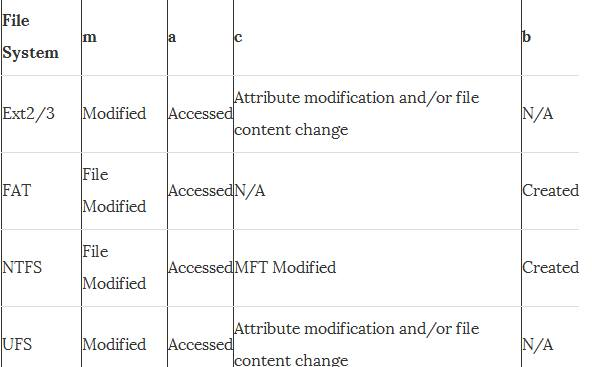
\includegraphics[width=0.7\textwidth]{graphics/mactime}
	\caption{MacTime}
	\label{fig:Mactime}
\end{figure}

\begin{figure}[tbph]
\centering
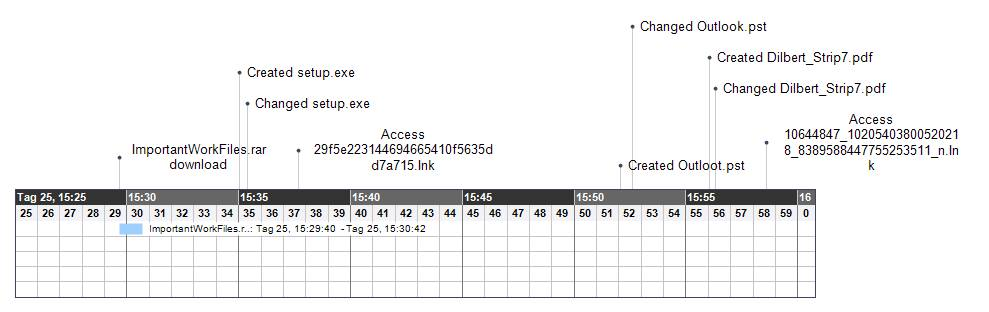
\includegraphics[width=0.7\textwidth]{graphics/timeline}
\caption{Timeline}
\label{fig:timeline}
\end{figure}

\section{Further techniques}
There are several other ways to handle and analyze encrypted data. Proper encryption is not easy and it can be time-consuming, especially if not the whole system is encrypted but individual files. In this section we describe further techniques to to retrieve passwords, data and metadata to and from encrypted files.
\subsection{Social engineering and retrieving passwords}
Maybe the easiest way to obtain passwords to encrypted data is to ask the suspect to reveal it or to offer a decreased sentence in exchange for the passwords.
This should be considered especially when the data retrieved through decryption could be used as digital evidence in other cases.
In case the suspect is indeed innocent, he is likely willing to give away his password to drop the charges against him.\\
In the united Kingdom, a organization or a person can be required to reveal the password by law. This is because of the Part III of the Regulation of Investigatory Powers Act (RIPA), which is active since  the 1\textsuperscript{st} of October 2007.\cite{passwordsInUK}

Methods not covered by our experiment also include attacks directed towards the password, like Brute-Force attacks, rainbow-table attacks and dictionary attacks. These methods are using a list of already known passwords (rainbow-table, dictionary) or they are using all possible passwords (brute-force) in an attempt to find the right password or password hash.
To accelerate these methods, it is useful to create a list of potential passwords, custom-built to the suspect. While generating this list, it is recommended to include names, birth-dates of family members or pets and other information retrieved through social networks and the social environment of the suspect. During this reconnaissance of the suspect it is also useful to extract all strings from all the confiscated devices and use them as a list. This could be useful since the suspect might have written and saved the password at some point. In addition to that it could be useful to apply dumpster diving, that means to look for information in the dumpster of the suspect. 
The holy grail of dumpster diving is, to find the password written on a piece of paper. 
Aside that, there are already created lists with standard and often used passwords available.
While this could lead to the correct password and therefore to the immediate decryption of the data, these methods often require a big amount of
computing power and can take very long.
Especially the brute-force method should be only used, after all other ways to retrieve the encrypted data have failed.


\subsection{Retrieving the plaintext}
Sometimes the plain data can be obtained through several ways, for example the thumbnails of pictures like we showed during our experiment. This also includes intentional or unintentional Backups on internal or external devices and on cloud-systems.
This could be especially useful on devices where automatic synchronization with an online cloud exists (Dropbox, Google, Apple,...)google-cloud. Other places to look for include temp-folders, the history of certain programs used to open the files and system specific databases like the thumbnail databases under Windows.

\section{Conclusions}


\cleardoublepage{}
\printglossary[type=\acronymtype,title=Acronyms,style=long]

\printglossary[style=altlist,title=Glossary]

\bibliographystyle{acmdoi}
\bibliography{report}

\end{document}
